\chapter{Sensitivity Study and Results}\label{chapter:results}
The results section is divided into three sections: the sensitivity of the model-IIb are discussed, afterwards the take-off performance is discussed for the all engines operative, one engine inoperative and rejected take-off scenarios. Lastly, the balanced field length is discussed.

\section{Sensitivity Studies}\label{sec:sensitivitystudies}
Sensitivity studies are important because they give you insights into the magnitude of the impact that varying parameters can have on your design. Take-off performance is predominantly determined by wing design. The sensitivities of the take-off distance with respect to the thrust profile, $V_{lof}$ and air density are discussed. Furthermore, the rotation strategy -- described in \autoref{sec:rotation} -- has sensitivities with respect to $V_2$ and $s_{tofl}$ that should be inspected.  These sensitivities -- and others -- can evidently also be derived by differentiating the equations in \autoref{sec:verification}, since those models should respond in more or less the same way to an input change as the numerical model.

\subsection{Thrust Sensitivity}\label{sec:sensitivity_thrust}
Thrust is an important metric in aircraft performance. Often, thrust requirements are set by take-off performance requirements. Therefore, it is expected that the take-off performance is highly sensitive to the thrust-velocity envelope. Propeller thrust is essentially determined by propeller power and propeller efficiency. Changing propeller efficiency for the One Engine Inoperative (OEI) scenario has a significant impact on the take-off performance, as shown in \autoref{fig:sensitivity_efficiency_distance}. Clearly, designing a more efficient propeller can significantly lower the balanced field length. A more efficient propeller can also lower the required power if a take-off distance of, for instance, 2000 meters has been set in the take-off requirements.

\begin{figure}[!ht]
    \centering
    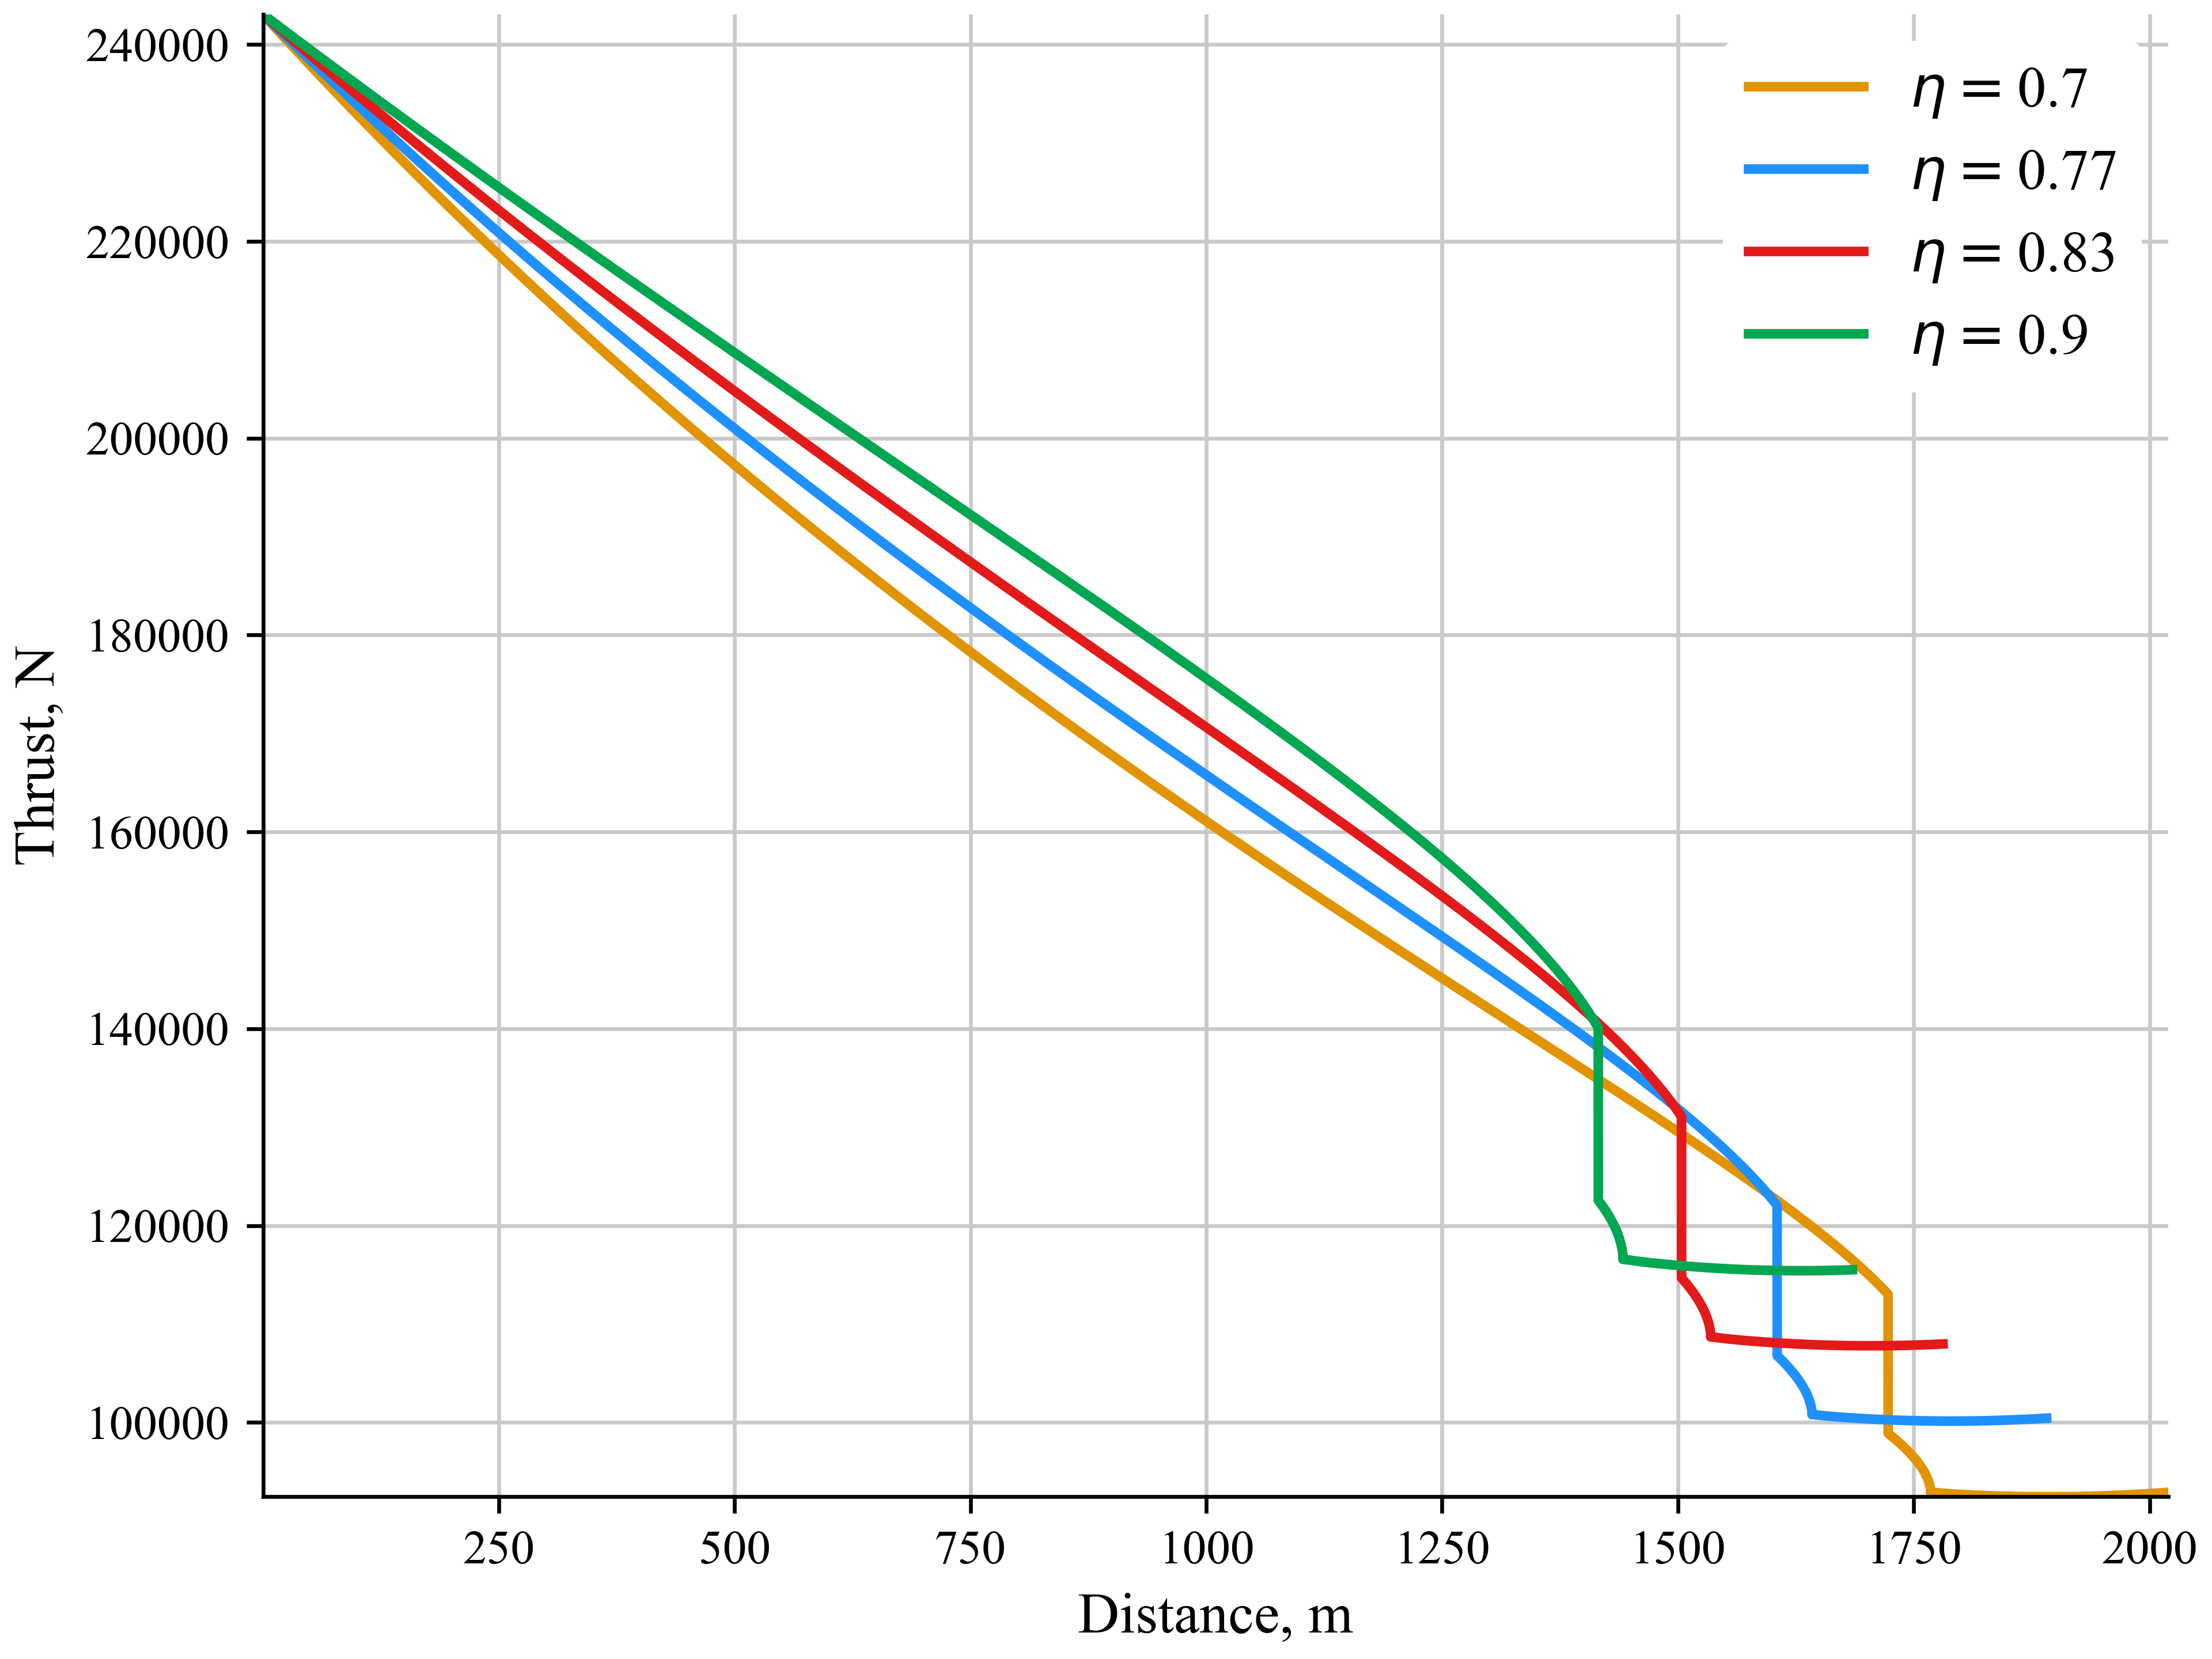
\includegraphics[width=0.5\linewidth]{figures/E9X_BFL_thrust_sensitivity.png}
    \caption{Sensitivity of propeller efficiency, and thus thrust, versus take-off distance for the E9X}
    \label{fig:sensitivity_efficiency_distance}
\end{figure}

\subsection{Lift-Off Velocity Sensitivity}\label{sec:sensitivity_Vlof}
The chosen $V_{lof}$ has a non-monotonous effect on the take-off distance. At first, increasing the $V_{lof}$ will decrease the take-off distance. After a certain $V_{lof}$-value, the take-off distance will increase. This decrease and increase can be seen in \autoref{fig:sensitivity_vlof_distance} for the Dash8-300. This may seem counter-intuitive at first, but since the take-off distance comprises of a ground-roll and airborne-phase, the one will increase as the other decreases. There is a point where the ground roll increases more than the airborne phase decreases however. This makes sense if you think about a limit cases: if the take-off velocity is incredibly high, the aircraft will almost instantly reach $h_\text{screen}$ as it rotates, but the ground roll takes a long time since it must reach that large $V_{lof}$ first.

\begin{figure}[!ht]
    \centering
    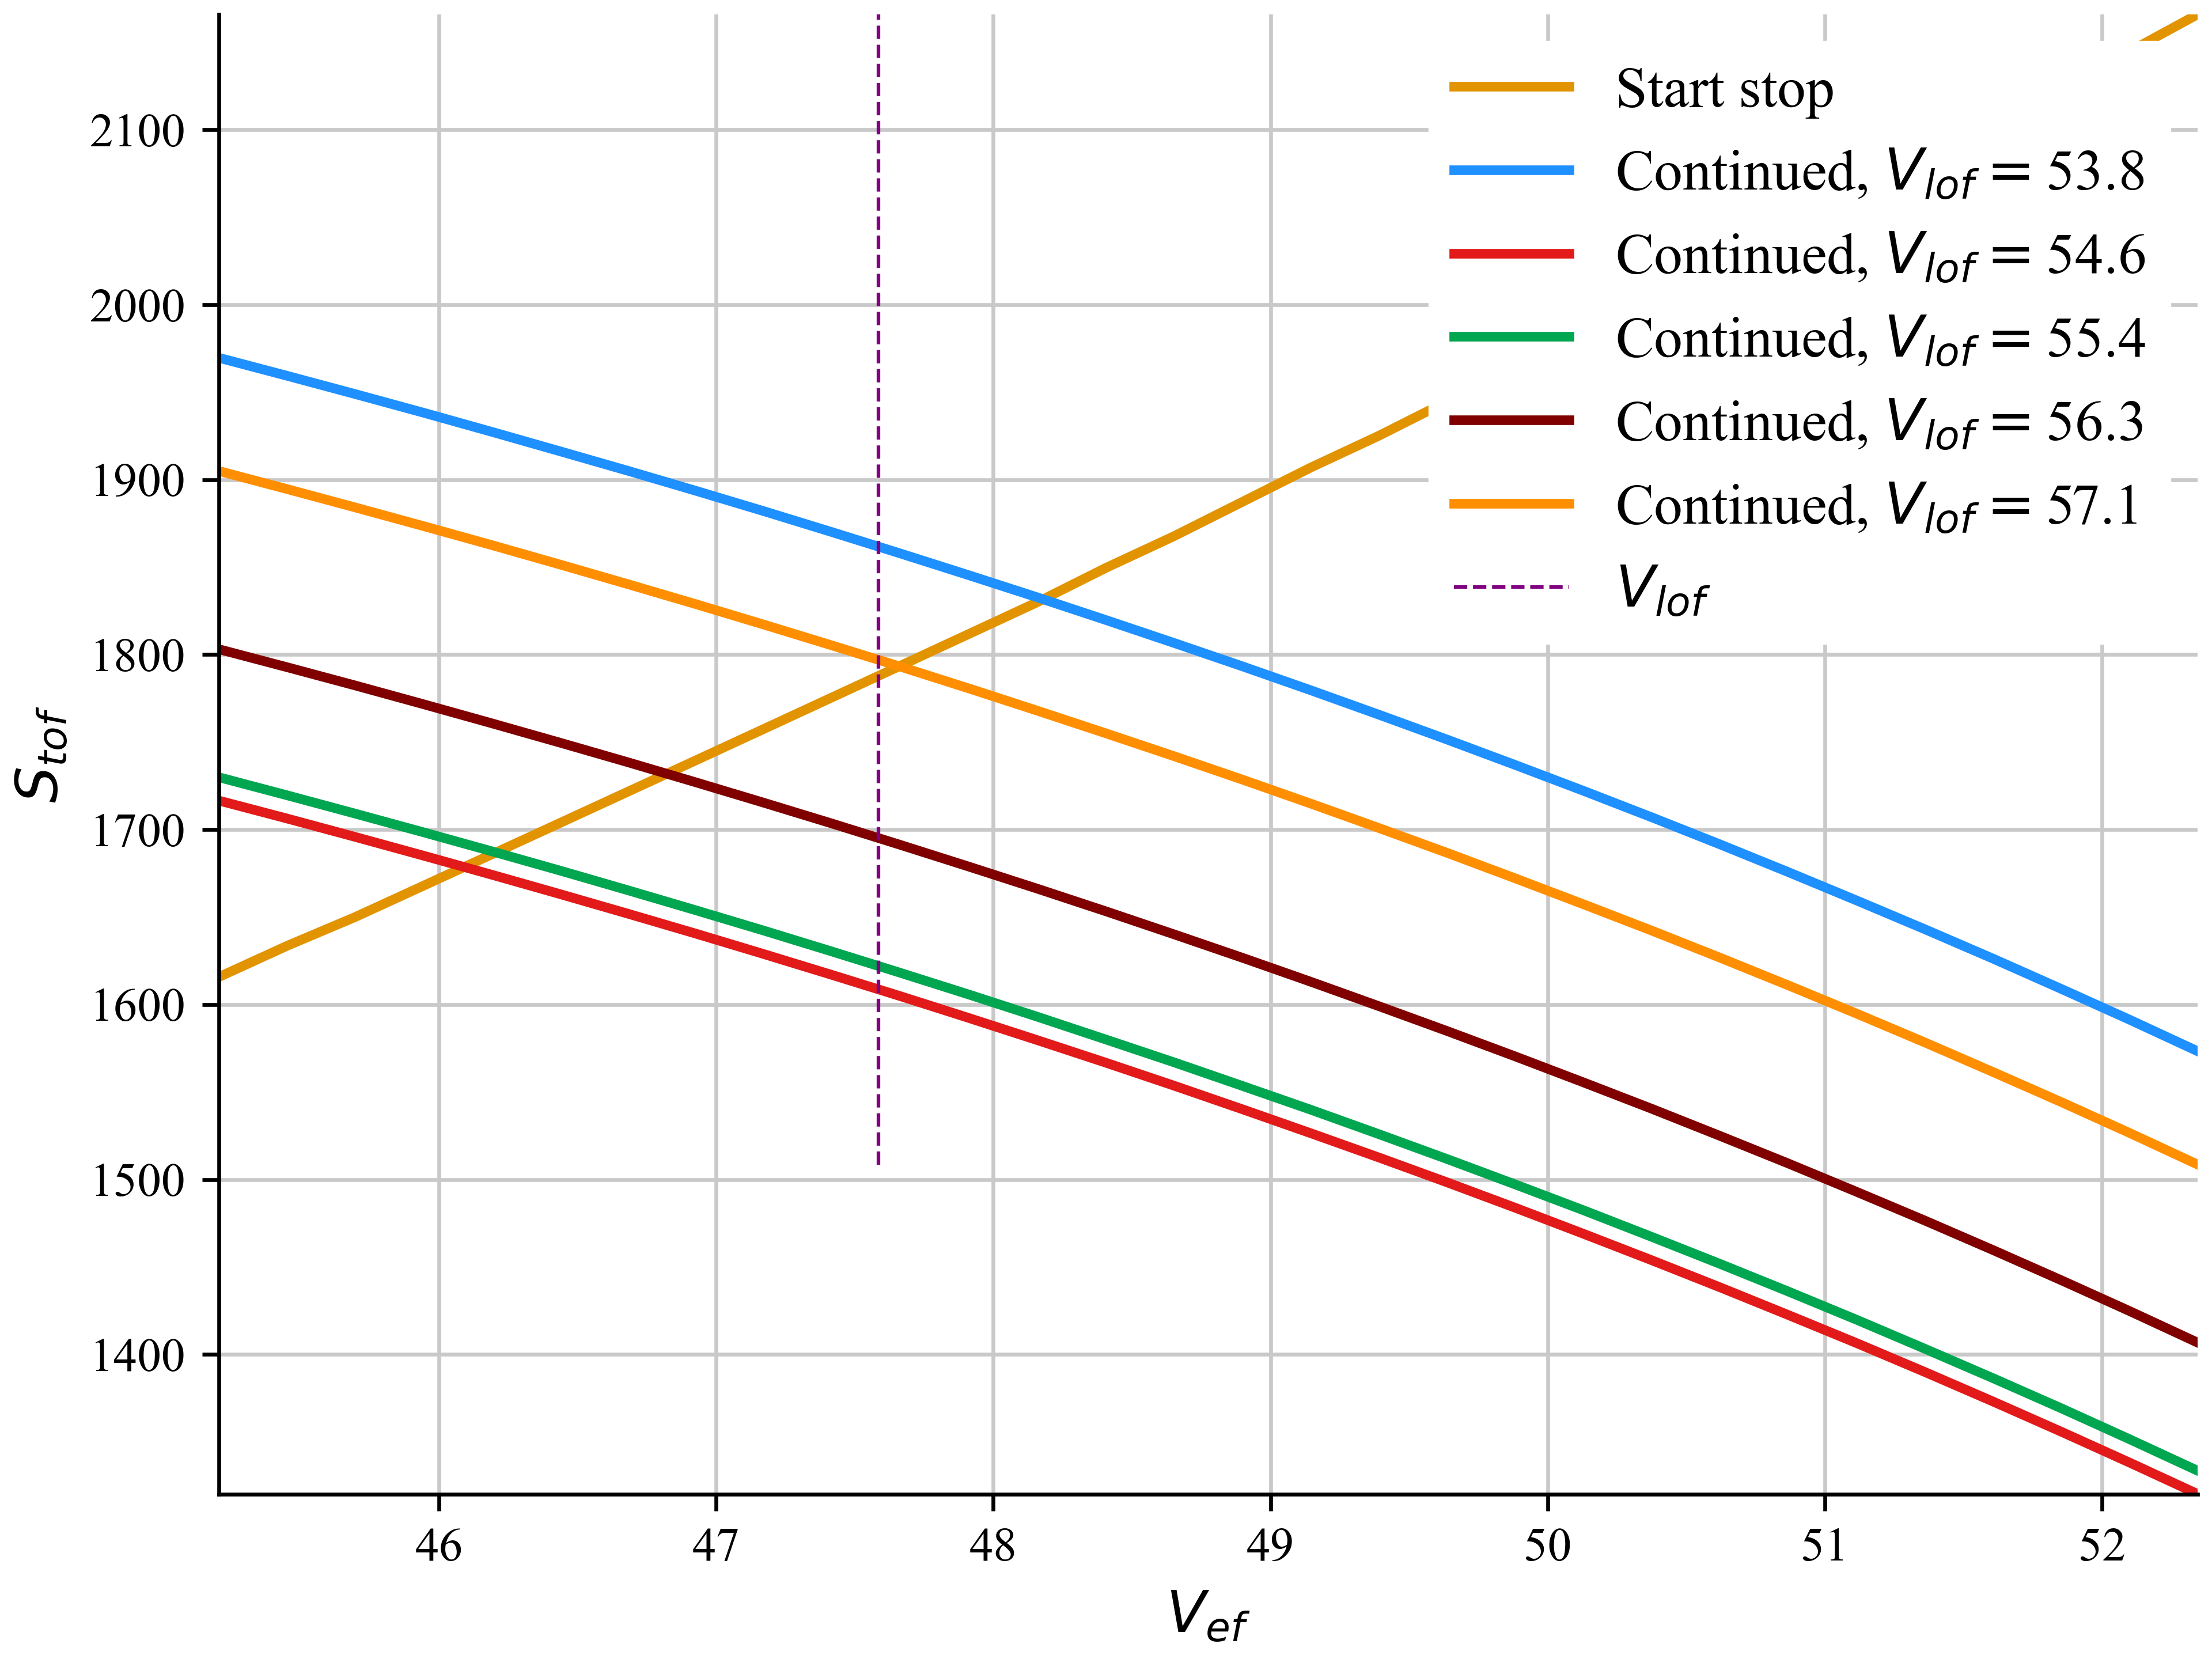
\includegraphics[width=0.5\linewidth]{figures/Dash8-300_BFL_Vlof_sensisivity.png}
    \caption{Sensitivity of $V_{lof}$ versus take-off distance}
    \label{fig:sensitivity_vlof_distance}
\end{figure}

\subsection{Rotation Strategy Sensitivity}\label{sec:sensitivity_rotation}
The last sensitivity that will be discussed in this section, is the relation between rotation speed (in degrees per second) versus take-off distance. The speed at which the aircraft rotates affects the airborne phase only. The faster a pilot rotates the aircraft, the quicker the $C_L$ will increase. Furthermore, it will pivot the engines in the $y$-direction, thus the (excess) thrust will also contribute to the vertical speed (and distance). As described by Torenbeek~\cite{torenbeek2013synthesis}, usually it is assumed that the rate of rotation is around 3-4 deg/s. In simplified analyses the angle of climb is usually determined using the excess power, or specific excess power. This approach was considered for a few weeks during this project as well and a model exists that uses this metric. It did prove to be counter-intuitive to use this metric in a time-stepping approach since the excess power existed in both directions. This meant that the authors tried to find a policy that produced a logical flight path and rotation pattern. Eventually, it was concluded that this approach -- for a time-stepping solution -- was convoluted and is thus not used in any of the models.

As expected, the take-off distance decreases with an increase in rotation speed. It also expected that there is a limit to the decrease, since the airborne phase will be zero at best -- leaving the ground roll unaffected.

\begin{figure}[!ht]
    \centering
    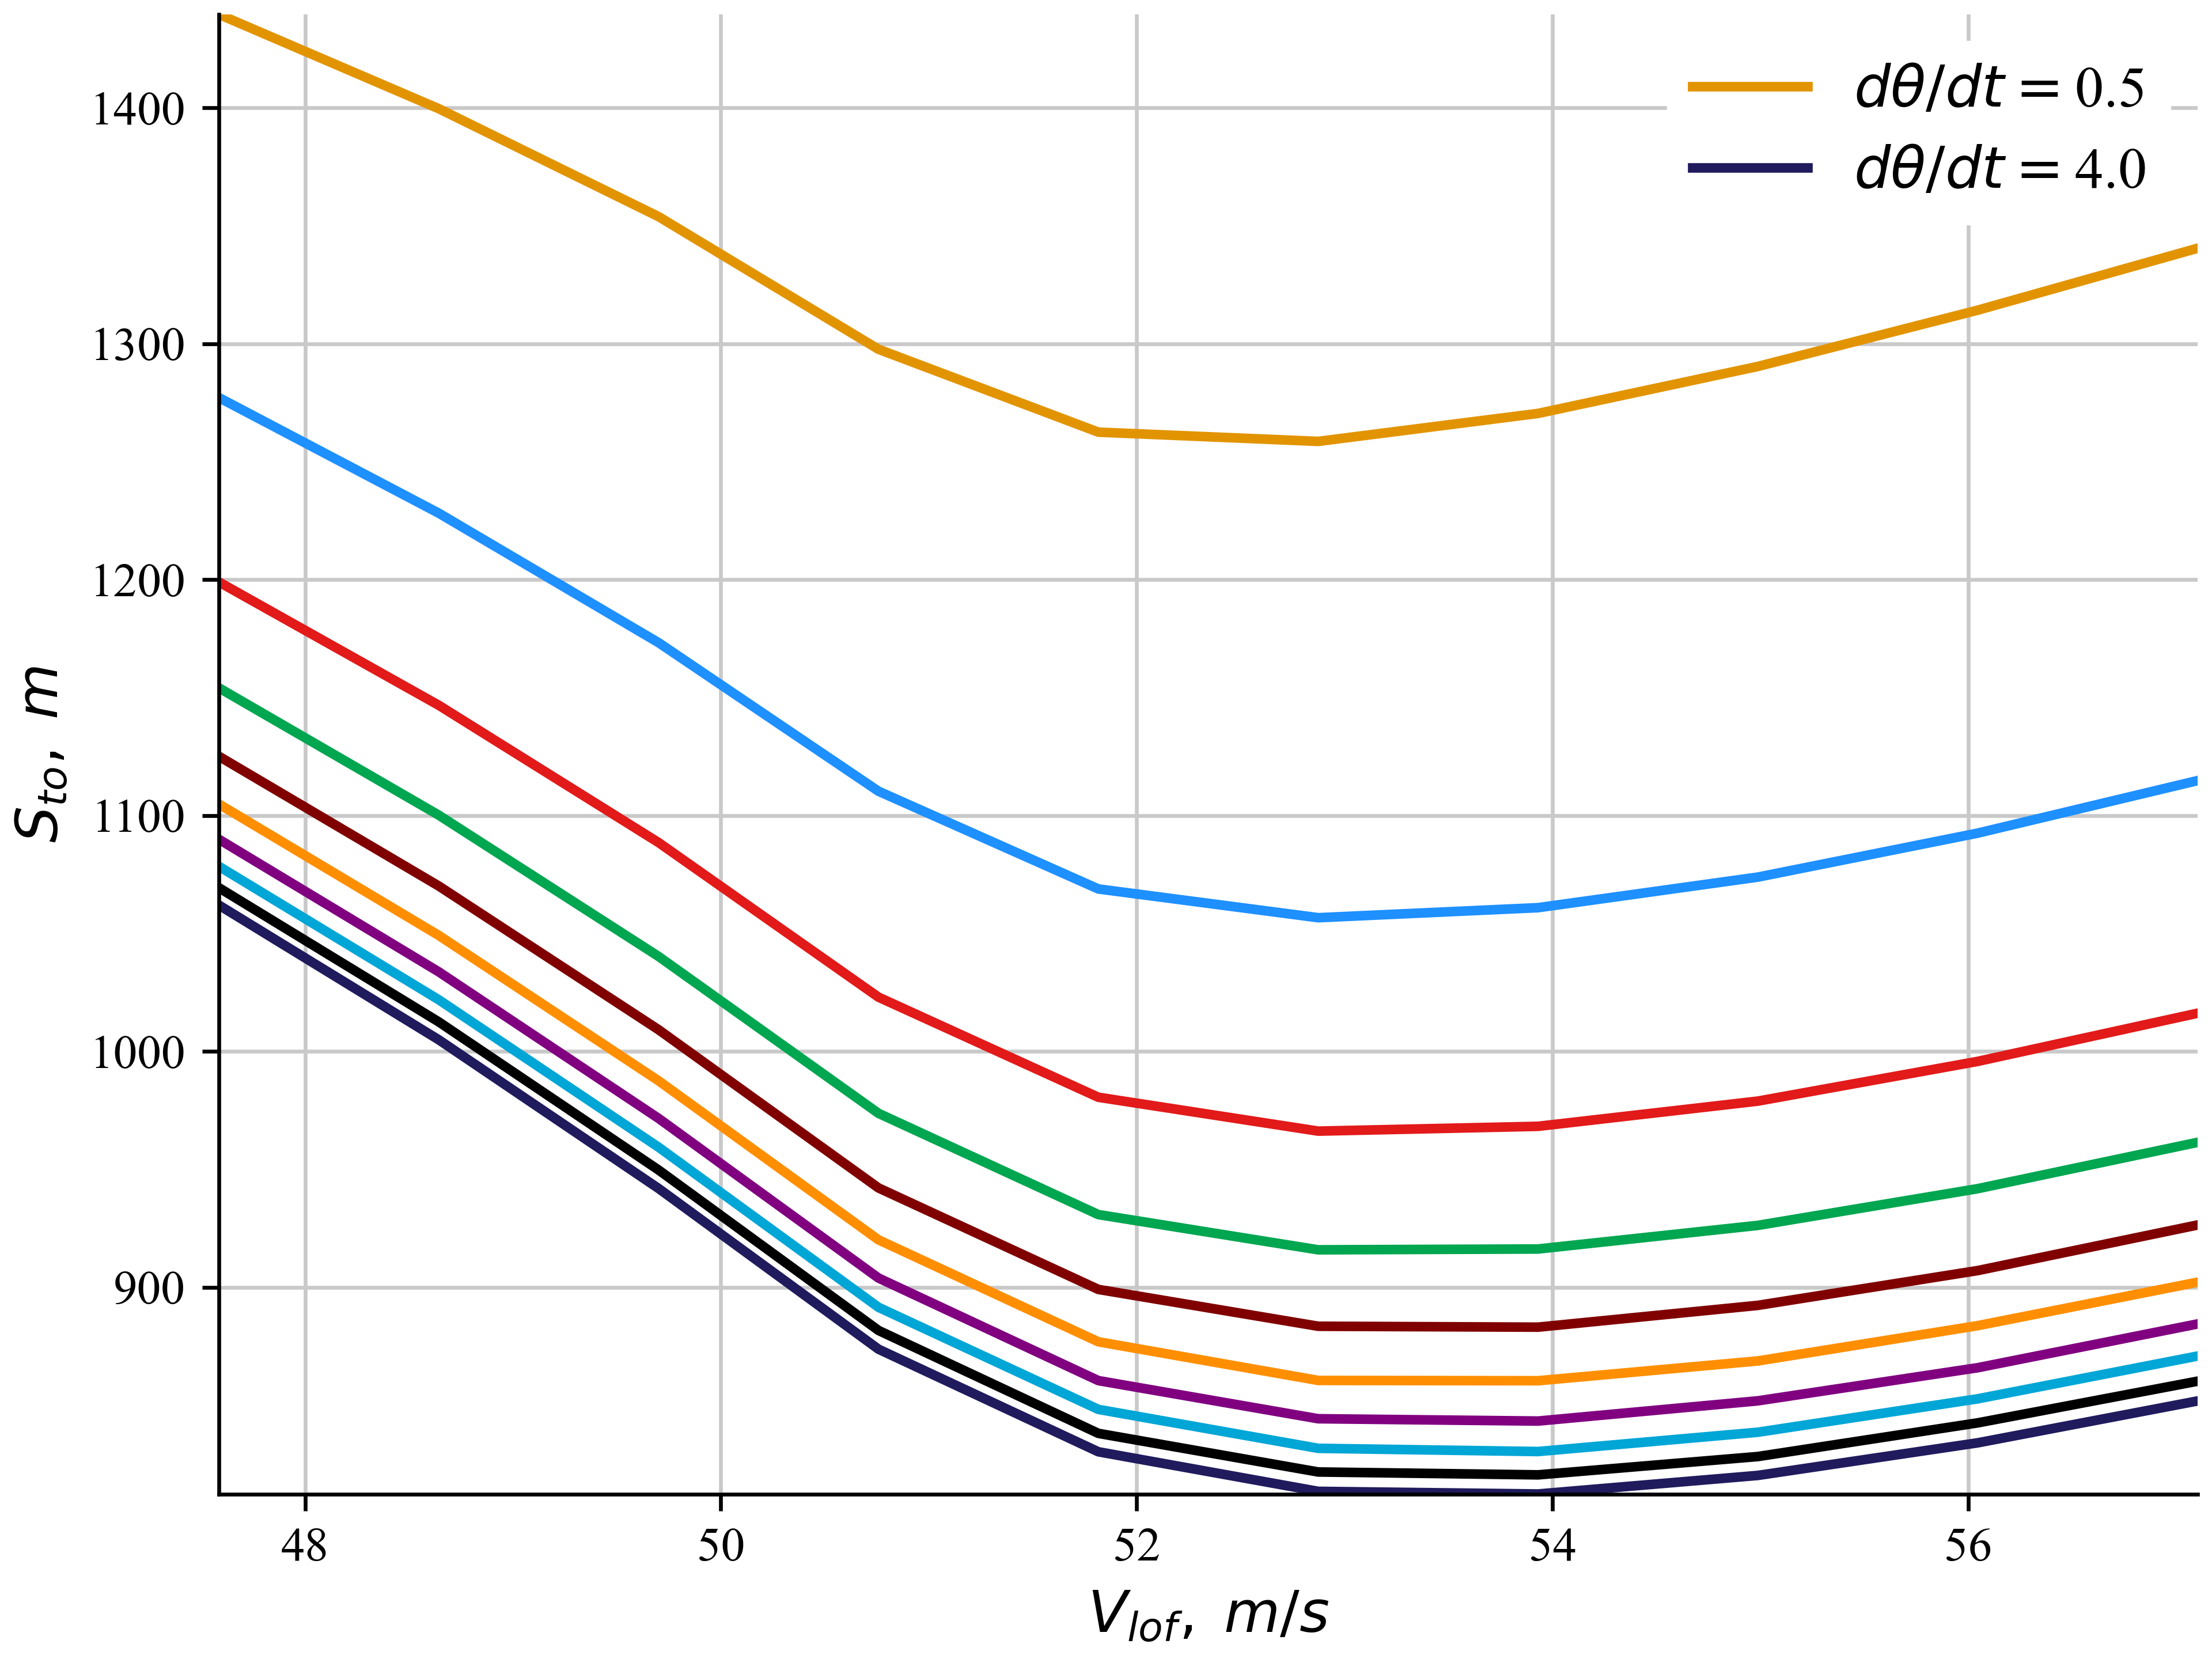
\includegraphics[width=0.5\linewidth]{figures/Dash8-300_takeoff_level2b_sensitivity.png}
    \caption{Sensitivity of $d\theta/dt$ versus take-off distance}
    \label{fig:sensitivity_dthetadt_distance}
\end{figure}

The rotation rate $d\theta/dt$ and climb angle $\alpha_{climb}$ affect the rotation- and airborne-phase of the take-off procedure. A higher rotation rate increases the height and vertical velocity faster. However, if a low $V_{lof}$ is chosen, it might mean that the $V_2>1.08V_s$ constraint is not met. The maximum climb angle will increase the achievable $C_{L,TO,max}$, but if the rotation rate is not sufficiently high, a system with a lower climb angle might perform better. These phenomena are exactly described by \autoref{fig:sensitivity_V2_stofl_dthetadt}, where the black dotted line represents the minimum $V_2$ required.

Looking at \autoref{fig:sensitivity_V2_stofl_dthetadt}, we can conclude that a higher $\alpha_{climb}$ with a higher $d\theta/dt$ always performs better. Logically this makes sense, since we prioritize vertical displacement over horizontal acceleration as quickly as possible. However, all solutions below the black dashed line are invalid since these do not meet the $V_2>1.08V_s$ constraint. We can however find the point that provide feasible solutions and draw a line between those points on the graph on the right. This procedure would show us what take-off distance are within the feasible region, ie 'above the line'. This process is shown in \autoref{fig:sensitivity_V2_stofl_dthetadt}. This analysis proves that the lowest $V_2$ returns the lowest take-off distance, given a certain $V_{lof}$ and rotation strategy. As we saw in \autoref{fig:sensitivity_vlof_distance}, the $V_{lof}$-$s_{tofl}$ relation knows an optimum.

\begin{figure}[!ht]
    \centering
    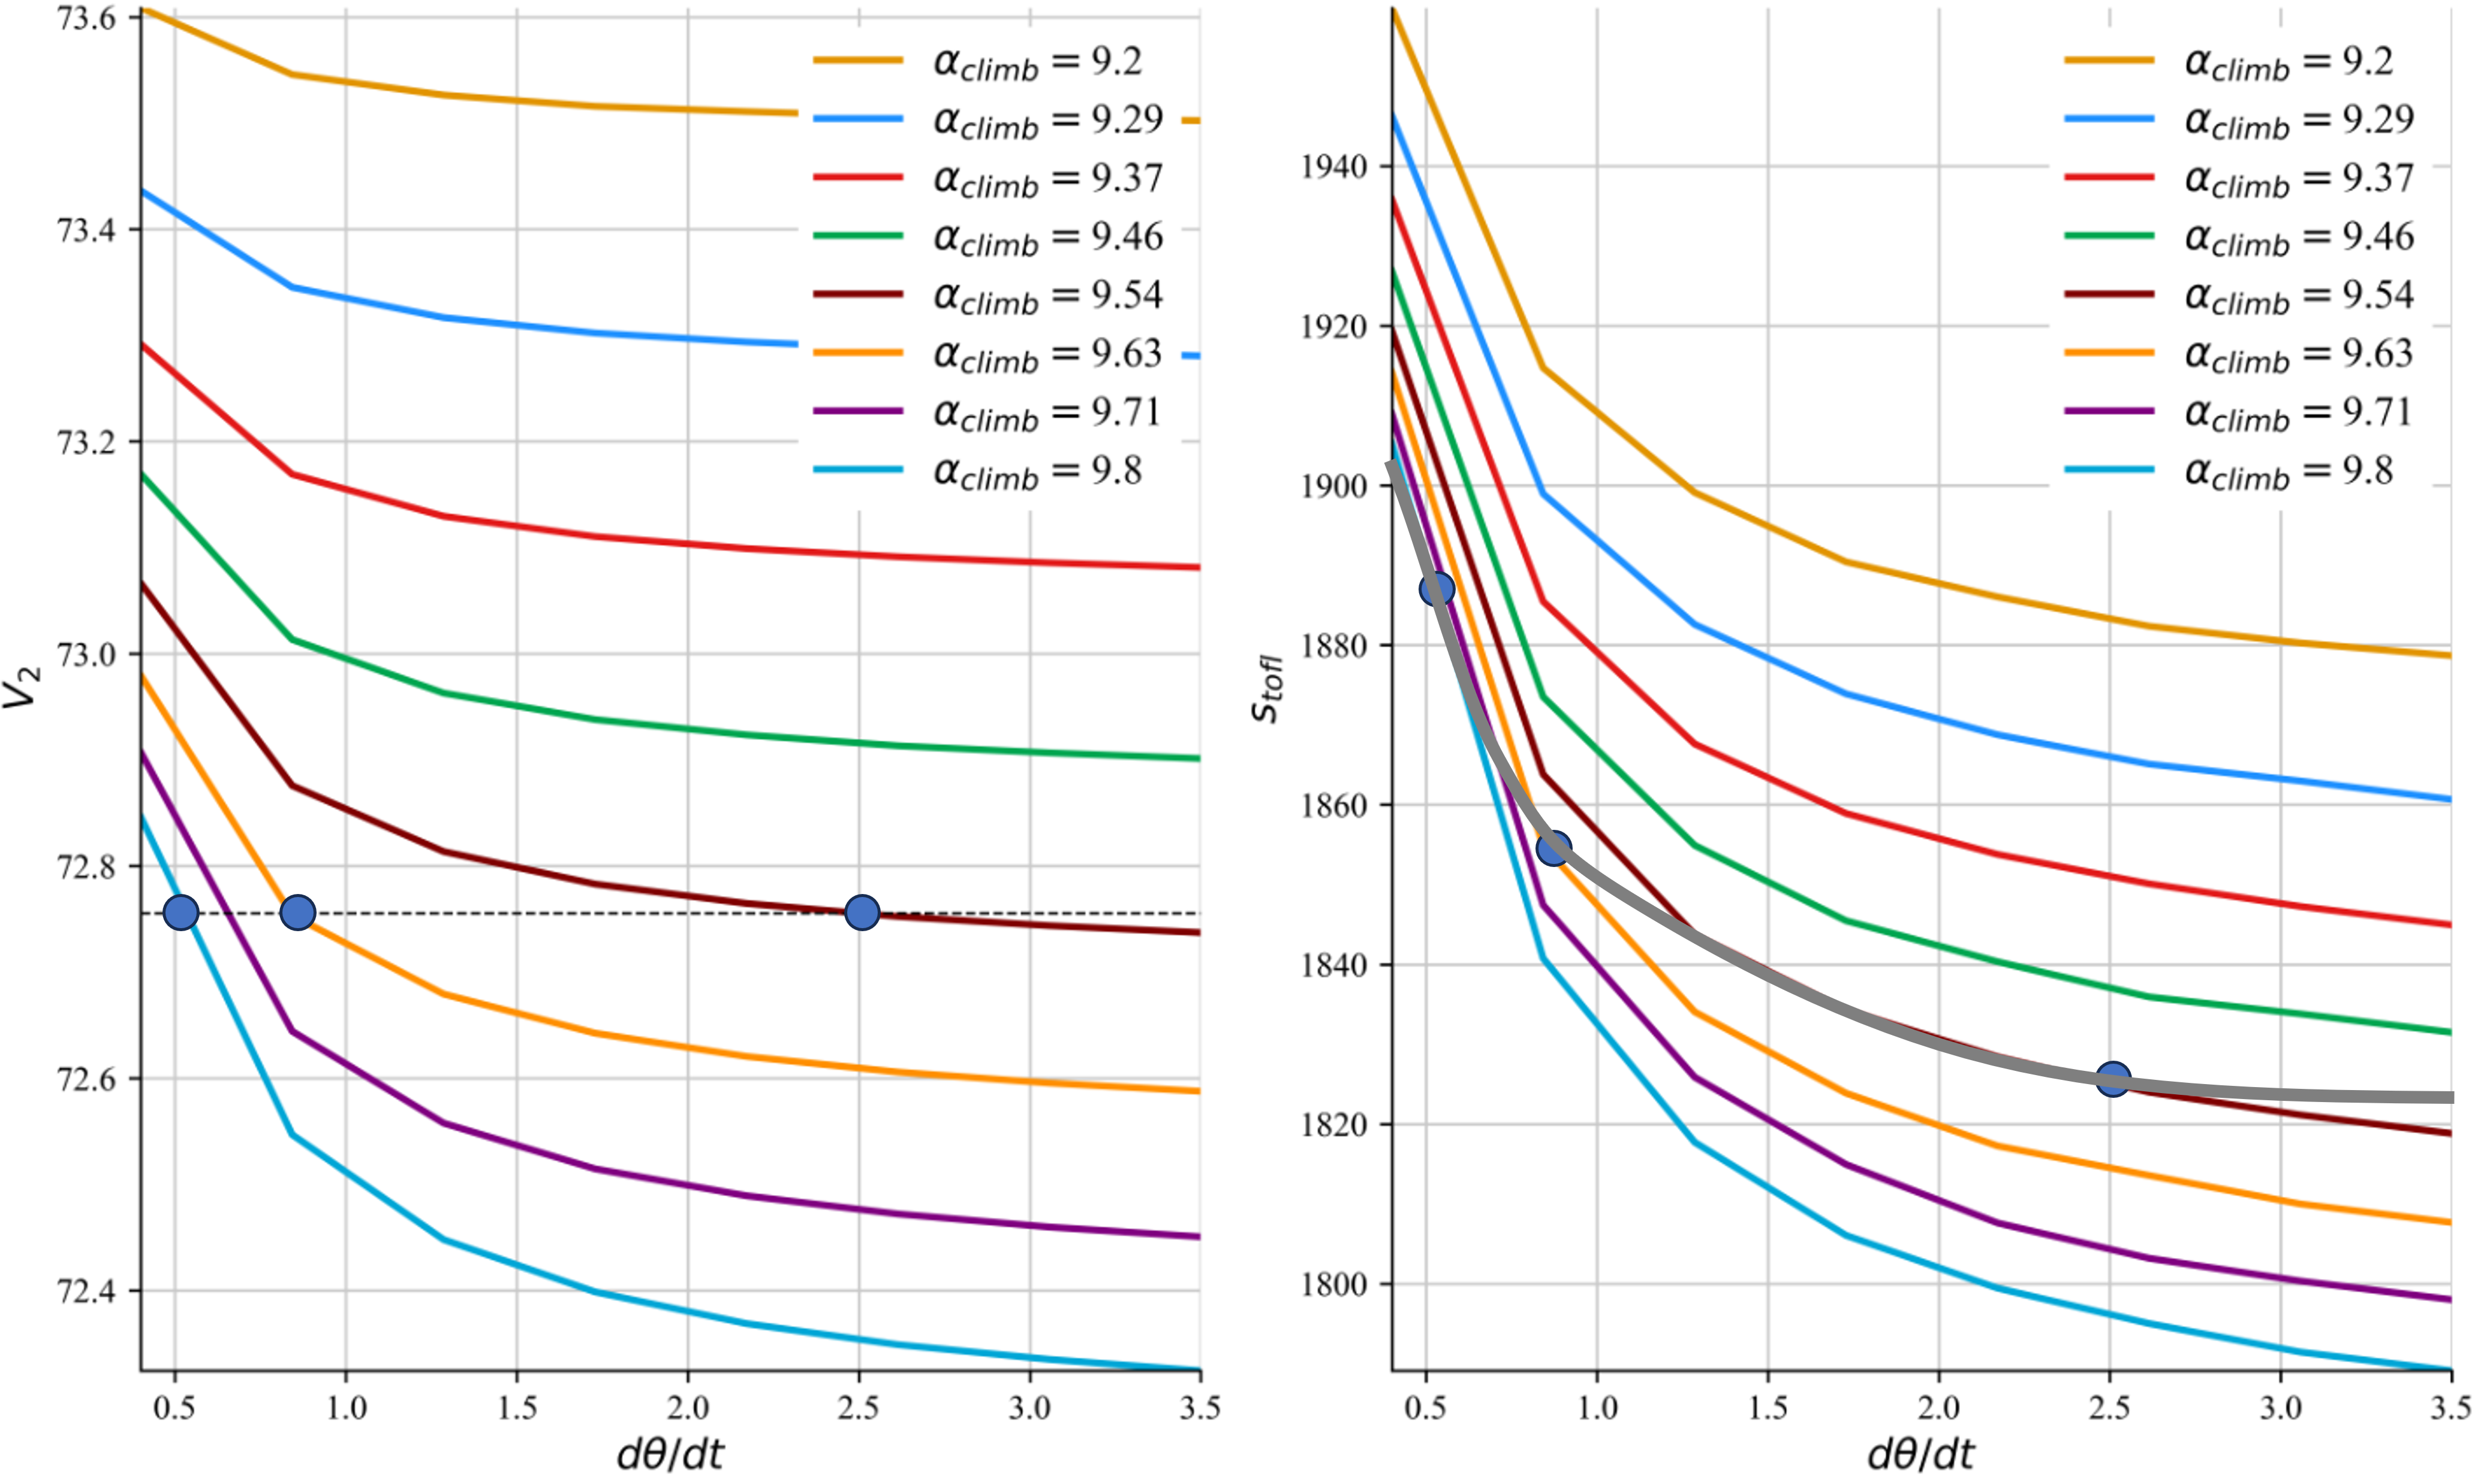
\includegraphics[width=\linewidth]{figures/takeoff_V2.png}
    \caption{Sensitivity of $d\theta/dt$ versus $V_2$ for several values of $\alpha_{climb}$ with a $V_2>1.08V_s$-constraint line}
    \label{fig:sensitivity_V2_stofl_dthetadt}
\end{figure}

\subsection{Ambient Conditions}\label{sec:ambientconditions}
Take-off distance also depends on ambient conditions. More specifically, the air density. Lowering density will increase the take-off density since stall speed increases. The sensitivity of take-off performance versus air density is given in \autoref{fig:sensitivity_density}. A decrease in take-off distance due to an increase in density is expected because the stall speed increases, and thus $V_{2,min}$ increases.

\begin{figure}[!ht]
    \centering
    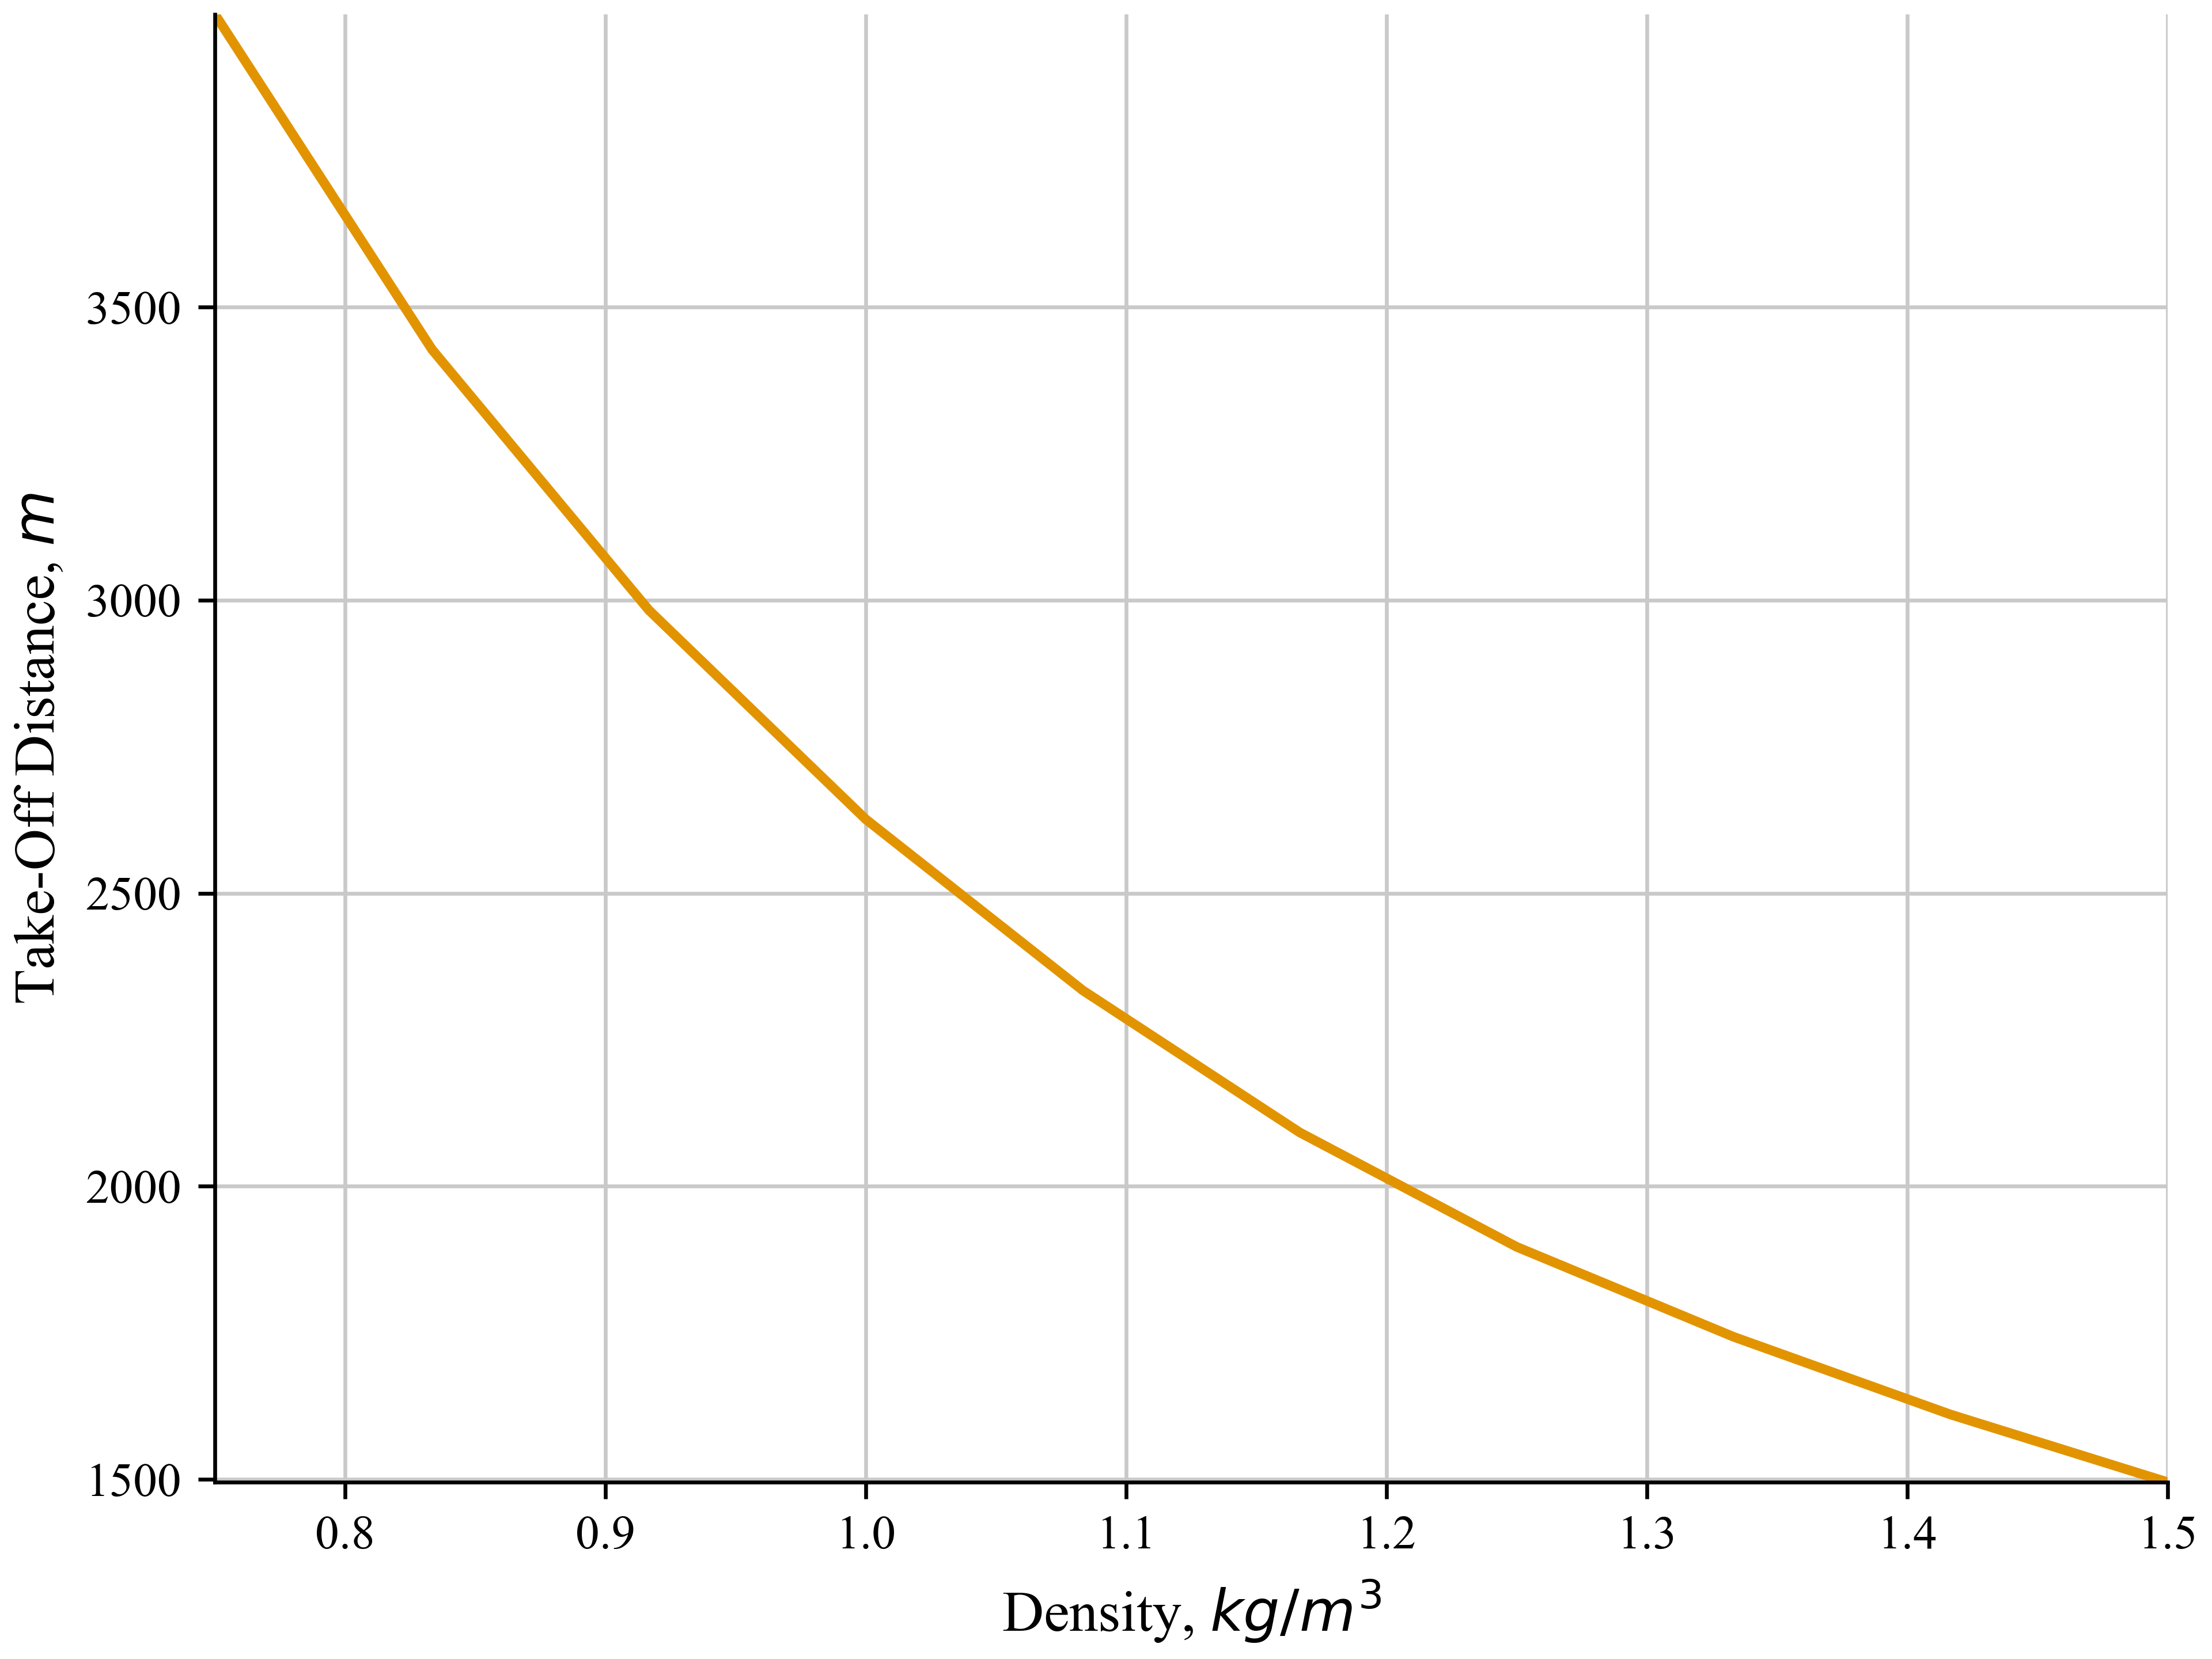
\includegraphics[width=0.5\linewidth]{figures/E9X_BFL_density_sensitivity.png}
    \caption{Take-off distance versus air density}
    \label{fig:sensitivity_density}
\end{figure}

\subsection{Pilot Induced Errors}\label{sec:piloterrors}
Human error could change the take-off requirements, by for instance rotating too late, too slowly or to a different climb angle than expected. The impact of such inaccuracies on the take-off distance and $V_2$ can be inspected by considering the system sensitivities given in the previous sections. 

The systems seems highly sensitive to changes in rotation rate, since it is hard to exactly rotate at a given rate. Similarly, the system is highly sensitive to changes in climb angle. The rotation rate and climb angle are inherently coupled. Consequently, a designer should consider a safety margin around these variables since small deviations could increase the take-off distance, or return a system that does not reach $V_2$. Lastly, $V_{lof}$ is analogous to $V_r$, and thus changing $V_{lof}$ is synonymous to rotating too late or too early. It seems like the system is less sensitive to this parameter when the designer chooses the optimal $V_{lof}$.

\subsection{Sensitivity Analyses Conclusions}\label{sec:sensitivity_conclusions}
These sensitivity analyses shows that an optimal take-off strategy exist. This optimal strategy can be achieved by carefully choosing $V_{lof}$, $d\theta/dt$ and $\alpha_{climb}$. Furthermore, optimizing the propeller performance during take-off can also have a substantial impact on the take-off performance. Lastly, it was confirmed that $V_{2,min}$ returns the smallest take-off distance.

\section{Take-Off Performance}\label{sec:takeoff_performance}
The take-off performance can be divided intro three sections: all engines operative (AEO), one engine inoperative (OEI) and the balanced field length. The latter is the most important for aircraft performance and sizing, since it is a key requirement. The former two give some insights into how the balanced field length could be shortened.

\subsection{All Engines Operative}\label{sec:AEO}
In case all engines are operative the take-off distance will be shortest. Furthermore, there is no instantaneous drop in thrust performance thus the take-off distance is more sensitive to design inputs such as propeller efficiency. A typical example of take-off performance for the E9X is shown in \autoref{fig:takeoff_AEO}. \autoref{fig:takeoff_AEO} conveys the system's information for all relevant parameters. It can be seen that the aircraft rotates until the maximum angle of attack and then stays there. Effectively, it means that the aircraft will keep rotating to compensate for the flight path increase. The graphs clearly indicate where $V_r$ and $V_{lof}$ occur, after which the vertical speed and displacement increase.

\begin{figure}[!ht]
    \centering
    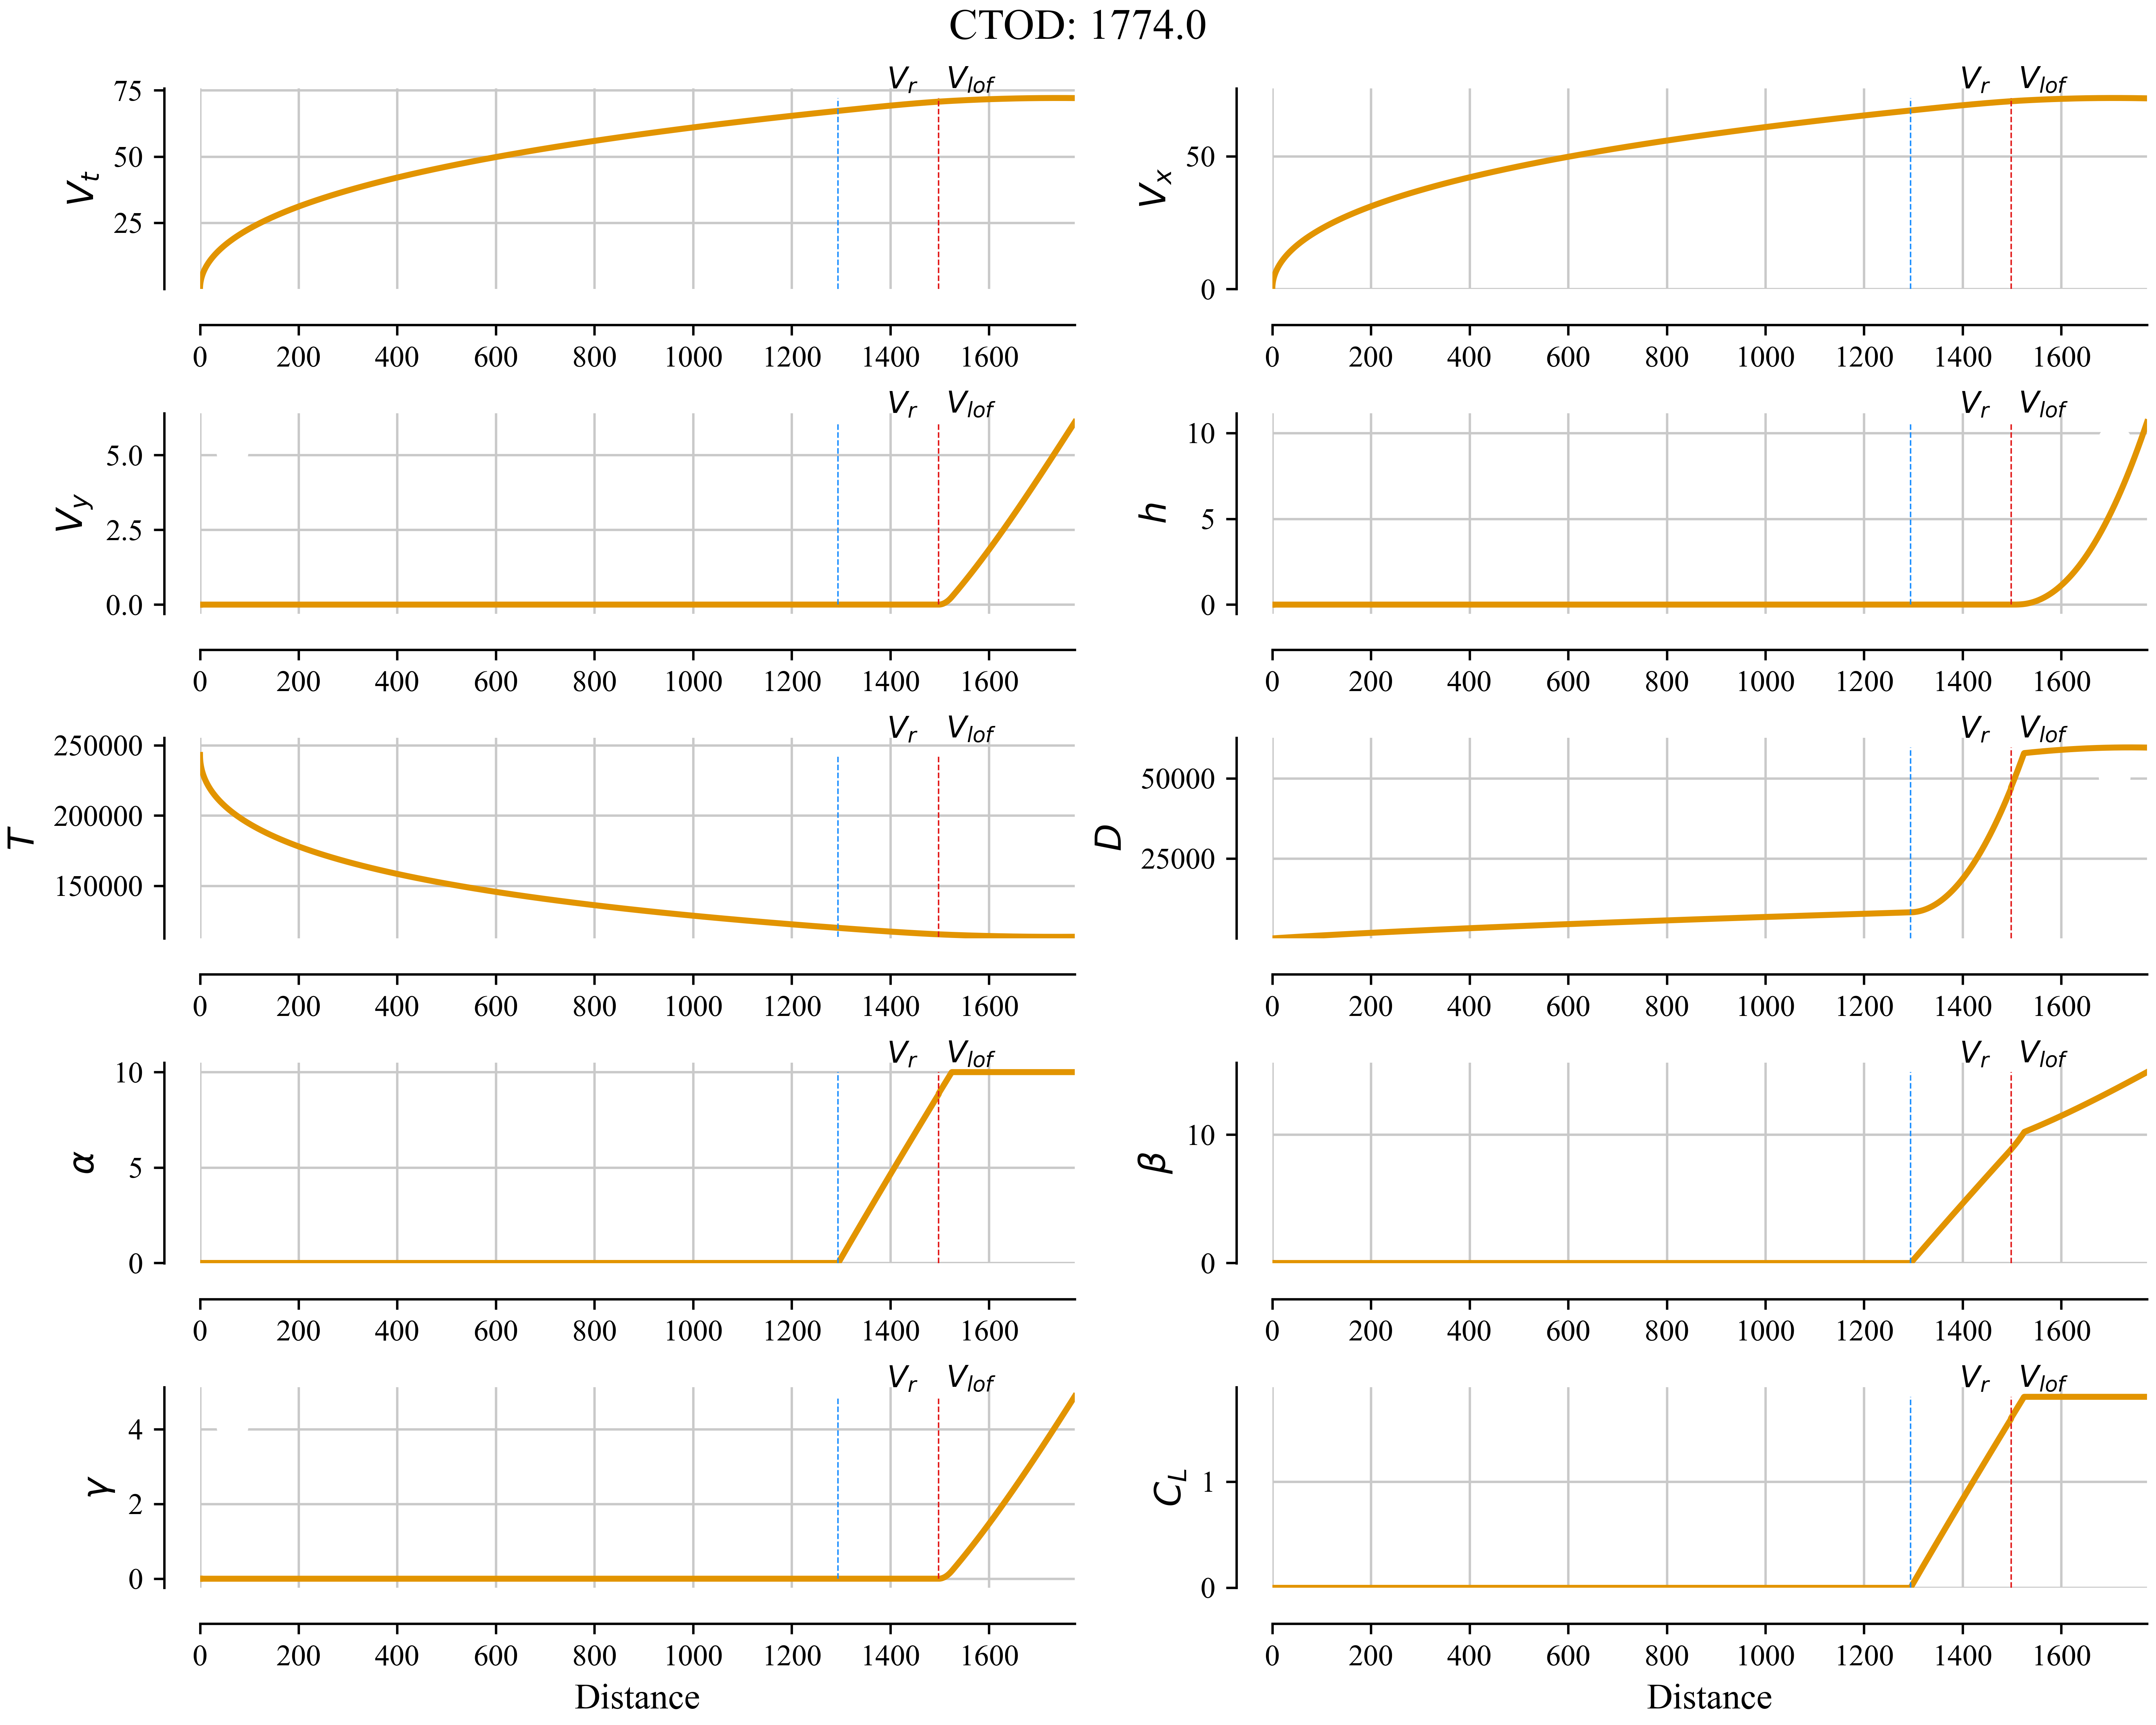
\includegraphics[width=0.8\linewidth]{figures/E9X_takeoff_level2b_ctod.png}
    \caption{Take-off performance for the E9X, AEO}
    \label{fig:takeoff_AEO}
\end{figure}

\subsection{One Engine Inoperative}\label{sec:AEO}
For the one engine inoperative case, engine failure occurs at the chosen $V_{ef}$. The continued take-off distance (CTOD) is the distance when the pilot would choose to continue the take-off. Due to the engine failure the take-off distance will be significantly longer, the $\alpha_{lof}$ changes and the $\alpha_{climb}$ changes, as compared to the AEO scenario.

\autoref{fig:takeoff_OEI} shows that one engine instantaneously stops working 2 seconds before $V_r$, thus causing a delay. Other than that, the curve is similar to the AEO case. All changes are linear and thus there aren't any major changes except for the take-off distance.

\begin{figure}[!ht]
    \centering
    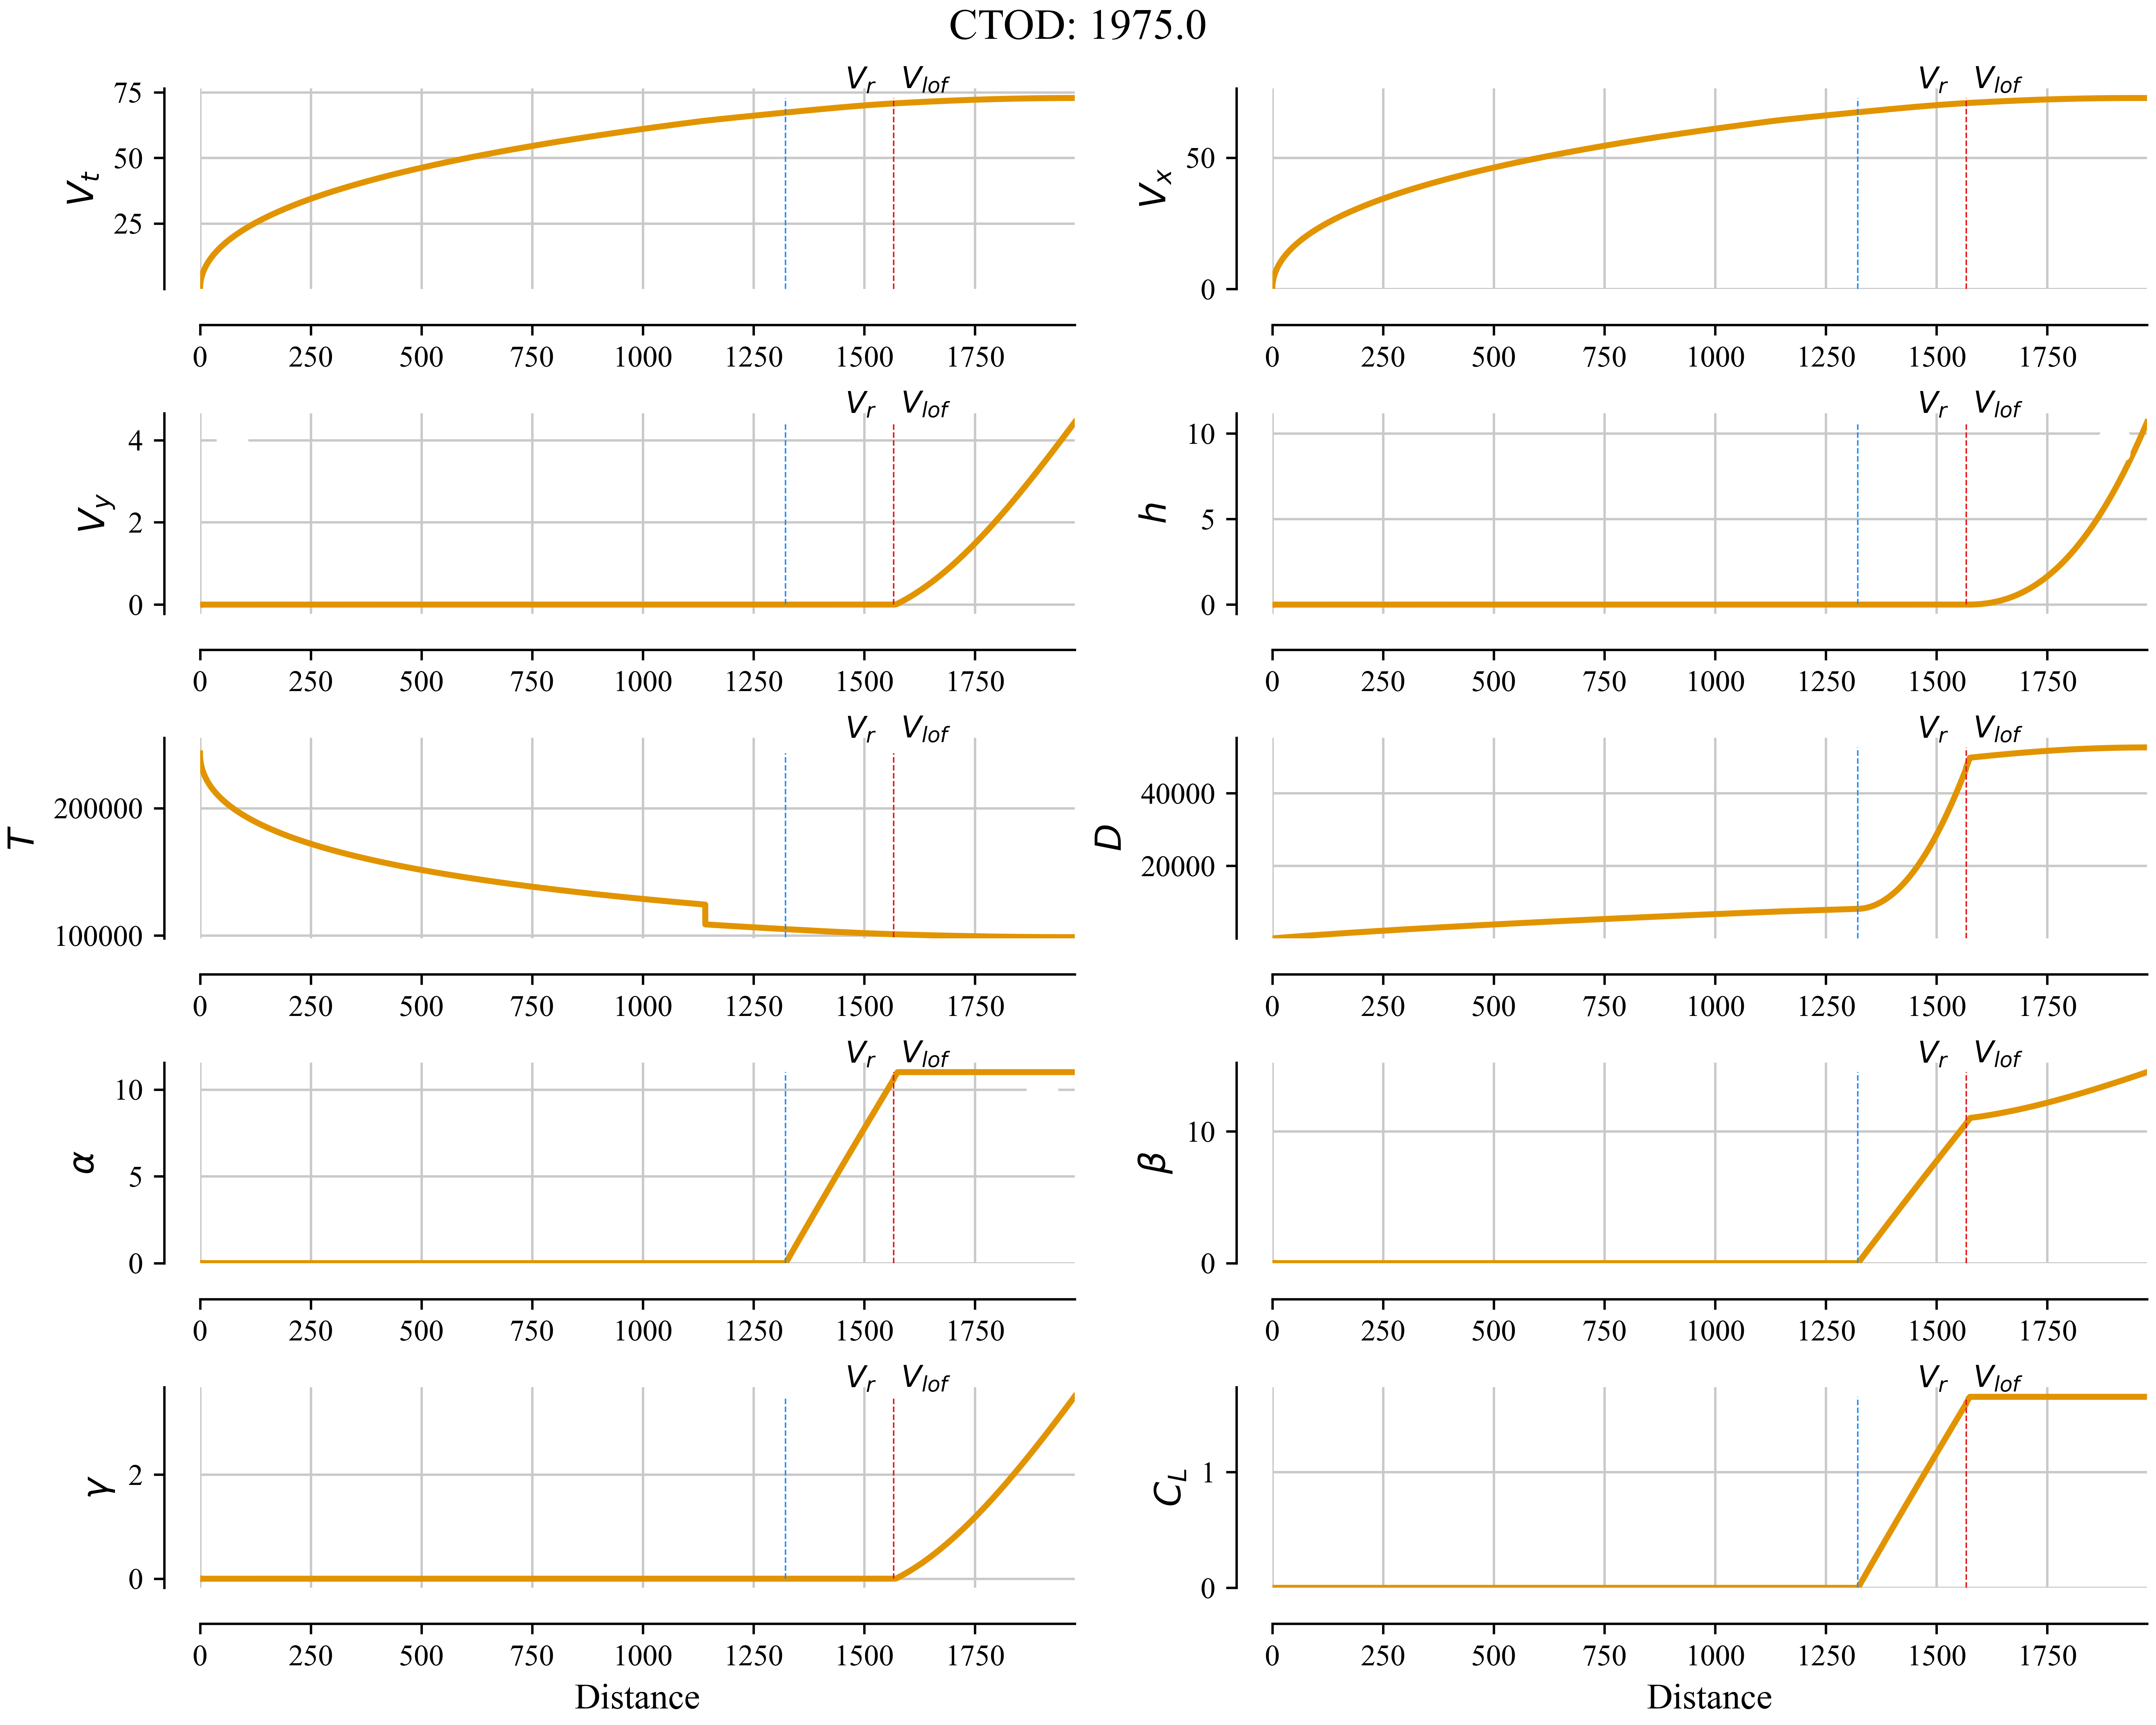
\includegraphics[width=0.8\linewidth]{figures/E9X_takeoff_level2b_ctod_OEI.png}
    \caption{Take-off performance for the E9X, AEO}
    \label{fig:takeoff_OEI}
\end{figure}

\section{Balanced Field Length}\label{sec:BFL}
As shown in \autoref{fig:schematic_takeoff}, balanced field length (BFL) is where the continued take-off and rejected take-off graphs intersect, since that's the shortest possible required runway. \autoref{fig:BFL} shows the BFL, expressed in take-off distance versus engine failure speed $V_{ef}$. The intersection in this graph happens around 1960 m, which therefore becomes the $s_{tofl}$. This results is in line with previous calculations, which estimated the BFL to be around 2000 m.

\begin{figure}[!ht]
    \centering
    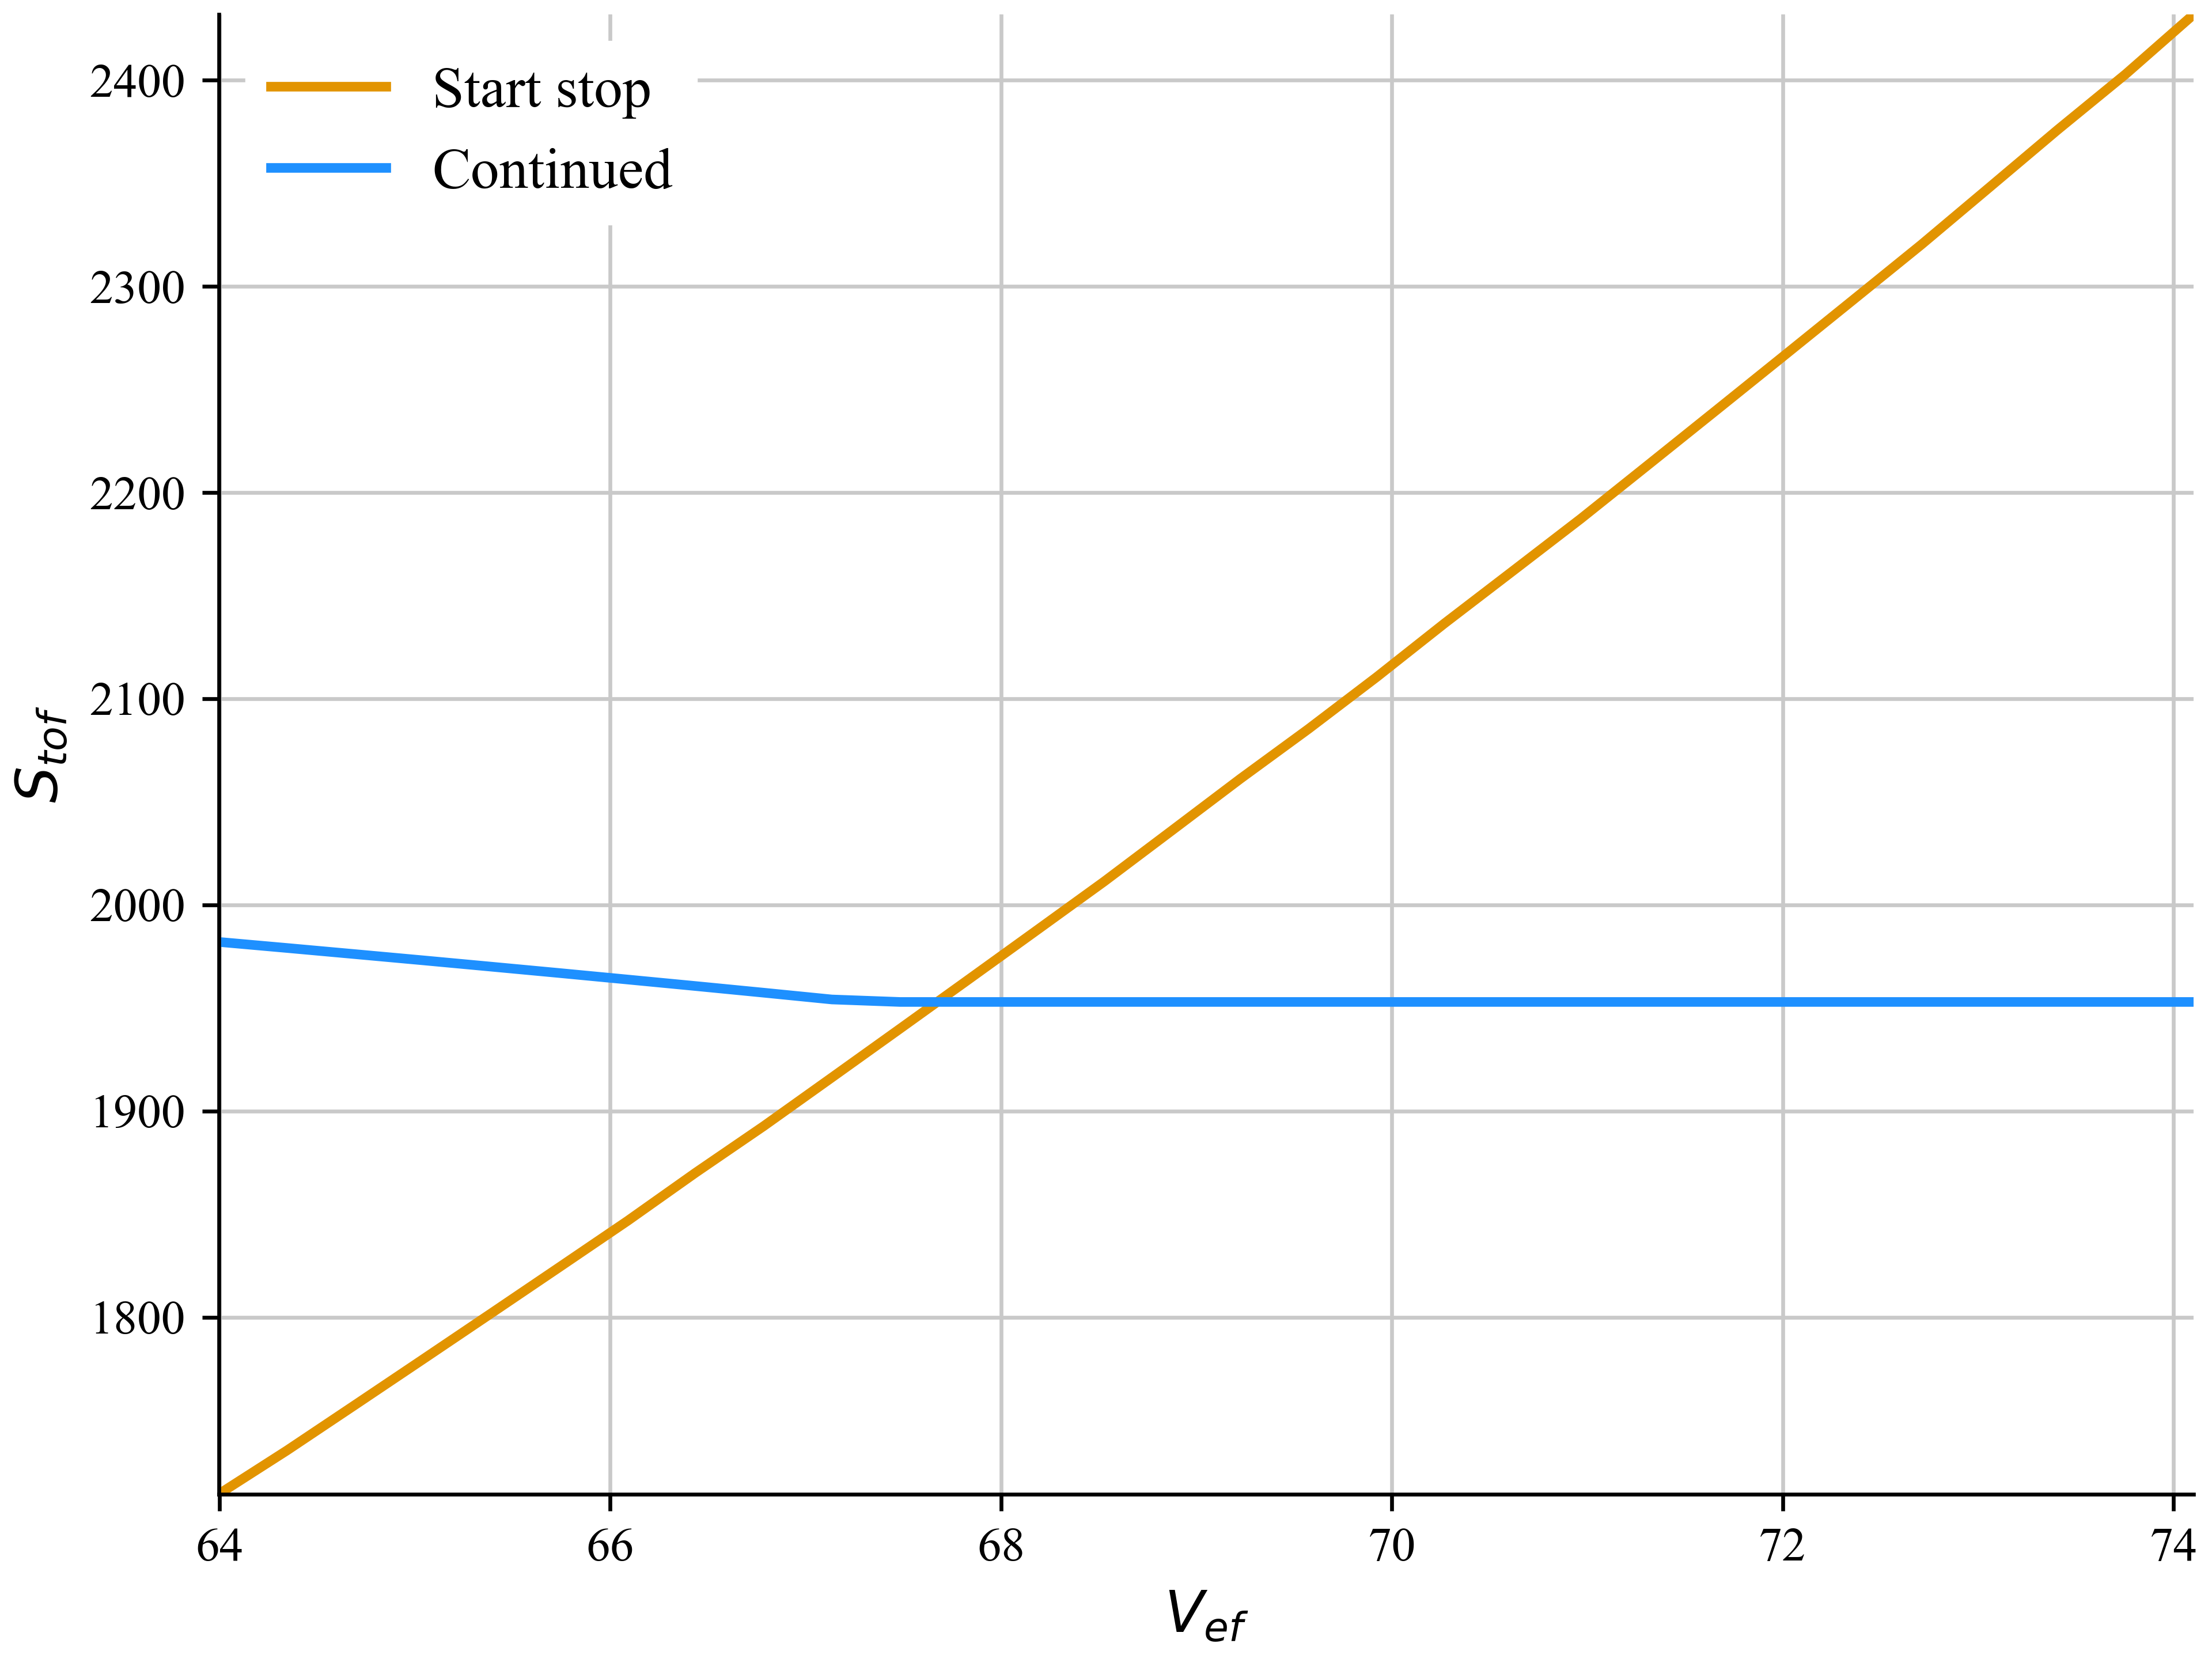
\includegraphics[width=0.5\linewidth]{figures/E9X_BFL.png}
    \caption{E9X BFL results}
    \label{fig:BFL}
\end{figure}
